
\chapter{Case Study}

\section{Jokela Town}

\section{Data}

%===============================================================
% Sanitary Sewer Inflow data
%===============================================================

    \subsection{Sanitary Sewer Inflow} \label{flowdata}
    
    \subsection{Meteorological Data}
    meteorological data is presented for both historical and forecast. 
    TELL HERE GENERAL THINGS ABOUT THE DATA THAT ARE EQUAL TO ALL SUBSUBSECTIONS I.E. THE PROVIDER, FORECAST MODEL, ETC.
        \subsubsection{Precipitation}
        Give characteristics of the data here, graphics and etc
        \subsubsection{Temperature}
        Give characteristics of the data here, graphics and etc
        \subsubsection{Temperature}

        
    \subsection{Topographic Data}
    DEM
    LAND USE
    URBAN AREA
    IMPERVIOUSNESS
    \subsubsection{Soil Superficial Deposits}
    
    The soil type coverage data was fetched from \acf{GTK} \cite{gtkdata} through its open data online service and was used to estimate the three parameters of Horton infiltration (see, \ref{infiltration}). The available information was obtained as vector data containing superficial deposits of Finland with material produced between 1972-2007. GIS operations were carried using Qgis to delimit the area concerned Jokela's catchment. Coverage of superficial deposit is depicted in figure \ref{fig:supdeposits}. Mixed soil types were simplified to facilitate model's parameter estimations.\\
    
\begin{figure}[h]
    \centering
	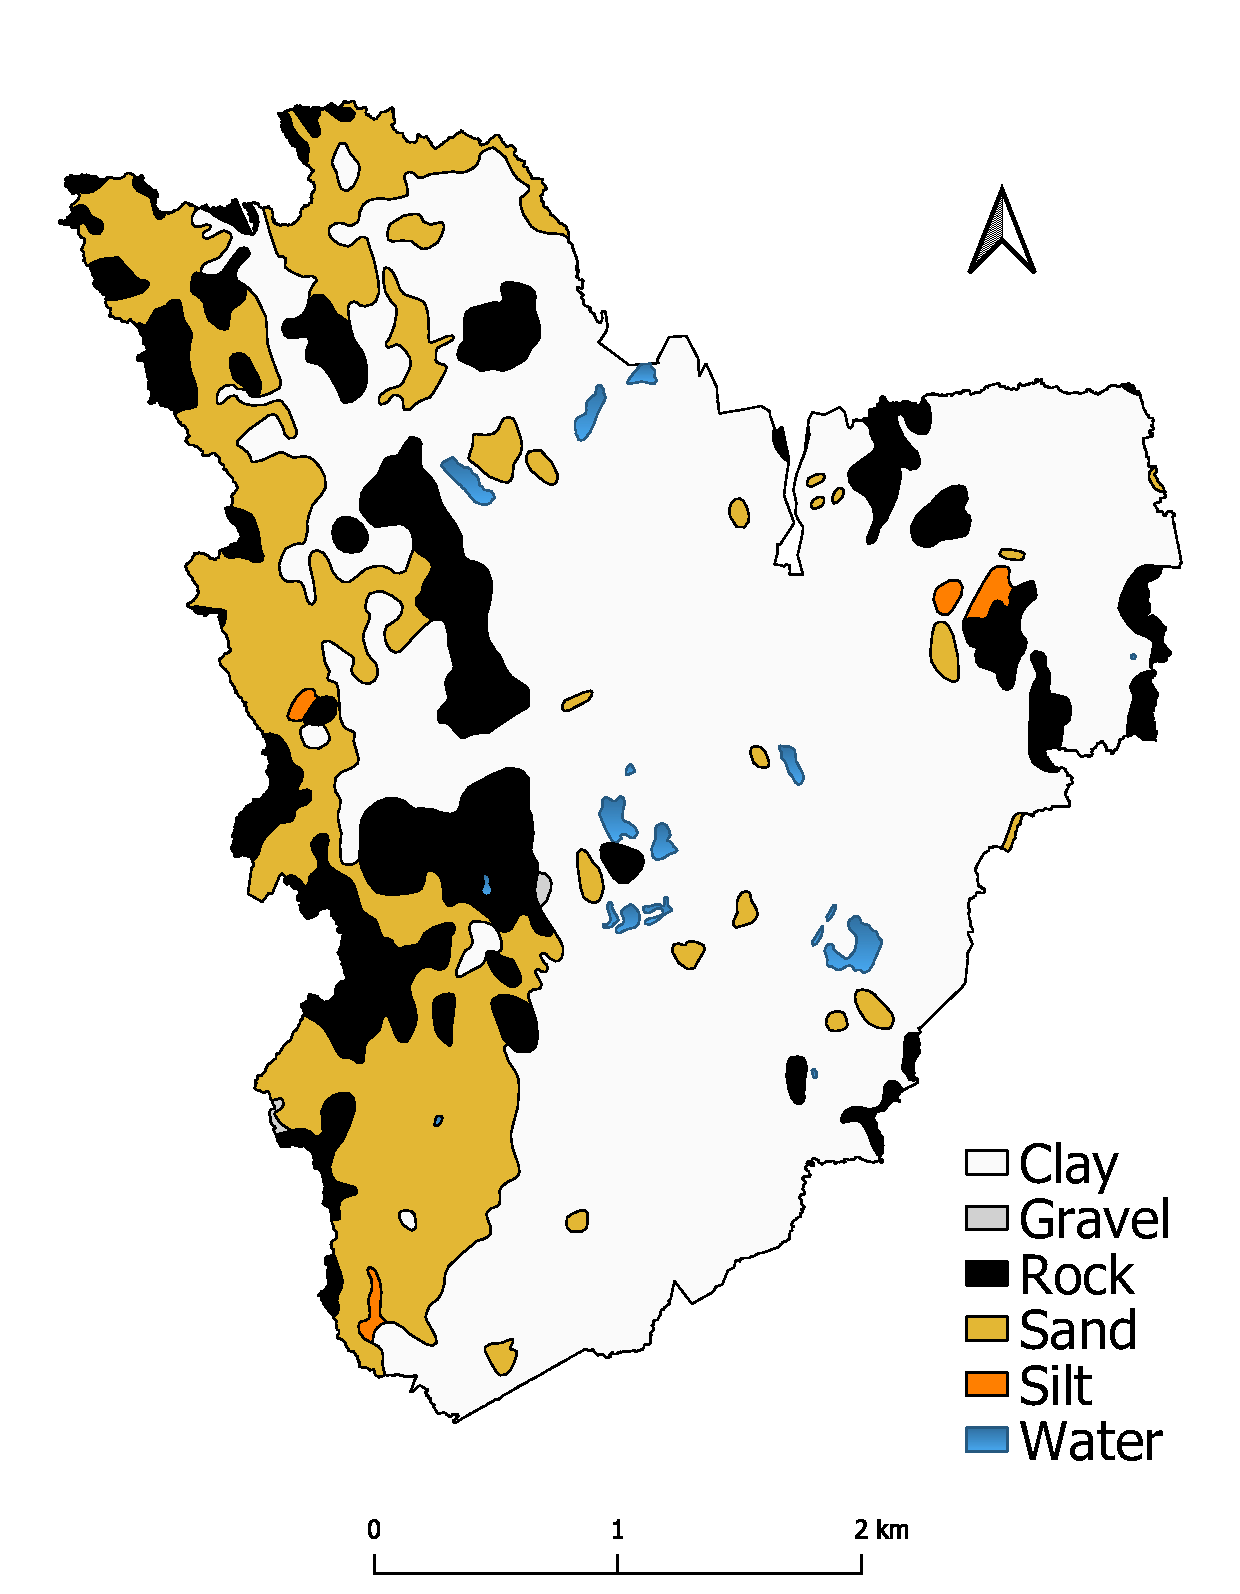
\includegraphics[scale=0.4]{figures/Jokela_Superficial_Deposits.pdf}
	\caption{Jokela catchment soil superficial deposits}
	\label{fig:supdeposits}
\end{figure}

As informed in section \ref{infiltration}, there are four parameters necessary to satisfy the Modified Horton infiltration model: Initial infiltration capacity ($f_0$); Minimum infiltration capacity ($f_\infty$), decay coefficient ($k_d$), and recovery coefficient ($k_r$) that is calculated based on drying time. For simplicity, the parameters were averaged by the whole area of Jokela catchment without considering subcatchment's divisions per pumping station. Therefore, all subcatchments have the same parameters for the infiltration model. Estimation of parameters was carried as follows:
\begin{enumerate}
    \item Initial infiltration capacity ($f_0$): values per soil type as estimated by \citet{Rossman2016} for DRY soils multiplied by 1.2 to account for vegetation present in the catchment.
    \item Minimum infiltration capacity ($f_\infty$): considered equal to saturated hydraulic conductivity with values estimated by \citet{Rawls1983} and available in SWMM user help.
    \item Decay coefficient ($k_d$): set to 4 [h\textsuperscript{-1}] as suggested by \citet{Rossman2016}.
    \item Recovery coefficient ($k_r$) in days: equation \ref{eqn:k_r} as function of minimum infiltration capacity in inches/hour.
\end{enumerate}

\begin{equation}
\label{eqn:k_r}
k_r = \frac{3.125}{\sqrt{f_\infty}}
\end{equation}


The estimation of each parameter for each soil type is depicted in table \ref{tbl:infparamest}. Area and percentage of coverage for each soil type was also calculated to spatially weight $f_0$, $f_\infty$, and $k_r$ using equation \ref{eqn:infilaverage} to obtain a unique value of each parameter to represent the entire catchment.


\begin{table}[h]
\caption{Modified Horton infiltration parameter estimation}
\label{tbl:infparamest}
\centering
\begin{tabular}{@{}lccccc@{}}
\toprule
\textbf{soil type} & \textbf{area [ha]} & \textbf{coverage [\%]} & \textbf{$f_0$} & \textbf{$f_\infty$} & \textbf{$k_r$} \\
\midrule
Clay               & 887.5                 & 66.0                       & 30.5          & 0.3                            & 28.8          \\
Sand               & 267.9                 & 19.9                       & 152.4         & 117.8                          & 1.5           \\
Rock               & 181.6                 & 13.5                       & 3.0           & 0.03                            & 90.9          \\
Silt               & 5.9                   & 0.4                        & 91.4          & 6.5                            & 6.2           \\
Gravel             & 1.2                   & 0.1                        & 1524.0        & 1180.0                         & 0.5           \\
Water              & 11.5                  & 0.9                        & -             & -                              & -             \\ \midrule
Total              & 1355.7                & 100.0                      & -             & -                              & - \\           
\bottomrule
\end{tabular}
\end{table}

\begin{equation}
\label{eqn:infilaverage}
Parameter = \sum_{n}^{m}(Parameter_n \cdot Coverage_n \cdot 0.1)
\end{equation}
where: \\
\indent $parameter$ = $f_0$, $f_\infty$ or $k_r$ \\
\indent $n$ = soil type (excluding water) \\

after applying equation \ref{eqn:infilaverage} was applied to the estimated parameters of table \ref{tbl:infparamest}. The result of $k_r$ was set to its upper limit range since it was greater than 14 days because of the predominance of soil types with relatively low saturated hydraulic conductivity (\textit{Clay and Rock}). The following unique parameters were obtained and included to SWMM model:

\begin{center}
  $f_0$ = 52.2 [mm/h], $f_\infty$ = 24.6 [mm/h], $k_d$ = 4 [1/h], $k_r$ = 14 [days]  
\end{center}





%===============================================================
% Groundwater case study
%===============================================================
\subsection{Groundwater} \label{gwcs}

As mentioned in the literature ((Bennett et al. 1999; Vallabhaneni and Burgess 2007), (Barden et al. 2011), and others), infiltration into the sewer lines can be caused by the seasonal elevation of groundwater table or other condition that increased soil moisture content causing a temporary saturated zone. Elevation of the groundwater table around Jokela town was assessed in this section as an attempt to identify a possible correlation with seasonal variations of the water table and the flow measurements of the town’s sanitary sewer network. 
Information of water table levels was provided by the Finnish Environmental Institute (SYKE) through its open data service (“Finnish Environment Institute (SYKE) Open Environmental Information Systems” n.d.). Data of three observation wells were available surrounding Jokela town as depicted in Figure 4. The recording period and routines among the three stations varies considerably - from one record per month to one record per year.

Picture

Measurements from 2004 to 2016 from station 0118651 -located southeast from Jokela- were combined and plotted in Figure 5. Years with less than six months recorded were left out: 2007; 2008; and 2017. All the eleven years records showed an elevation on the groundwater table from March to May. 

Picture

Only yearly measurements were available for the closest station 0154356 located around 5km west from Jokela. The records are from different months, mostly during spring and summer. Therefore, assessment of monthly variation for the same year was not possible. However, the available data suggests slightly higher water table levels on average from January to June for the period of 1999-2017.

Picture

The closest observation well with data available from 2018 was 110651. Measurements from 2018 were relevant to compare with flow measurements of the same year in the sewer network. As depicted in Figure 6, the groundwater elevation period is on average from February to May. Similar pattern as observed for station 0118651. For 2018, periods of February-March and April-May were presented elevation in the groundwater table. If a similar groundwater elevation pattern also occurred for Jokela town in 2018, located 9 km away, correlation between aquifer recharge periods and higher infiltration rates into the sanitary sewer exists. 
    
    
    \subsection{Weather Forecast}

\section{Data Treatment}

\section{Snowmelt and Rainfall for calibration and validation}



remind: Importance to use radar data and refer the literature vallabhnai conclusions of using radar and pawel nawalani that compared radar x rain gauge. 

remind: put a graph of variations in precipitation and temperature to justify that more data should be assessed. 


\section{Jokela Sanitary Sewer Model}

    \subsection{Hydraulic Model}
    
    \subsection{Physically-Based: SWMM Modules}


        \subsubsection{Jokela Sewershed Delineation}

\texttt{\textit{Area}} is one of the parameters necessary for many SWMM modules as described in equations X, XXU,XX,XX, and table x x X of previous sections. The definition of the \texttt{\textit{Area}} parameter for \acf{SSN} is rather conceptually challenging since it is located under the surface. This is due the different components of \ac{WWF}: surface/direct flow or sub-surface/infiltration flow gradient and the area of influence of each of these two processes. Rain drop falling over a specific point on the surface. The drop can flow over the surface towards the direction of the steeper slope or infiltrate and then flow through the porous in the soil to a very different direction than . As 
Therefore, delineating the sewershed only the \acf{DEM} rainfall-runoff

The sewershed delineation is a discretization of the space domain. The area division that supplies water to to a specific point within the \ac{SSN}. When modeling natural rivers, this area is assumed as all regions where a rain drop would flow downstream following the soil surface slopes from high elevations towards the lowest parts due to gravitational force. This method, however, is not conceptually valid for \ac{SSN} once the network's slopes are not always as the terrain slopes. Therefore, \ac{SSN} has a different gradient than the surface in some parts and pumping stations are required to transport waste water towards the \acf{WWTP}. This is the reason why the space domain was discretized per pimping station in this study.


Two reasons:
- Terrain slope
- Available historical flow measurements.

Qgis application was chosen to perform GIS operations and delineate sewersheds due to its free open services. GRASS r.watershed. 


Pumping stations are usually located in areas with lower surface elevation when compared to its upstream pipe network to direct the flow utilizing gravitational force and reduce energy consumption. However, differences between soil surface and network still exists in some parts of the pumping station upstream service area. 


\begin{figure}[h]
    \centering
	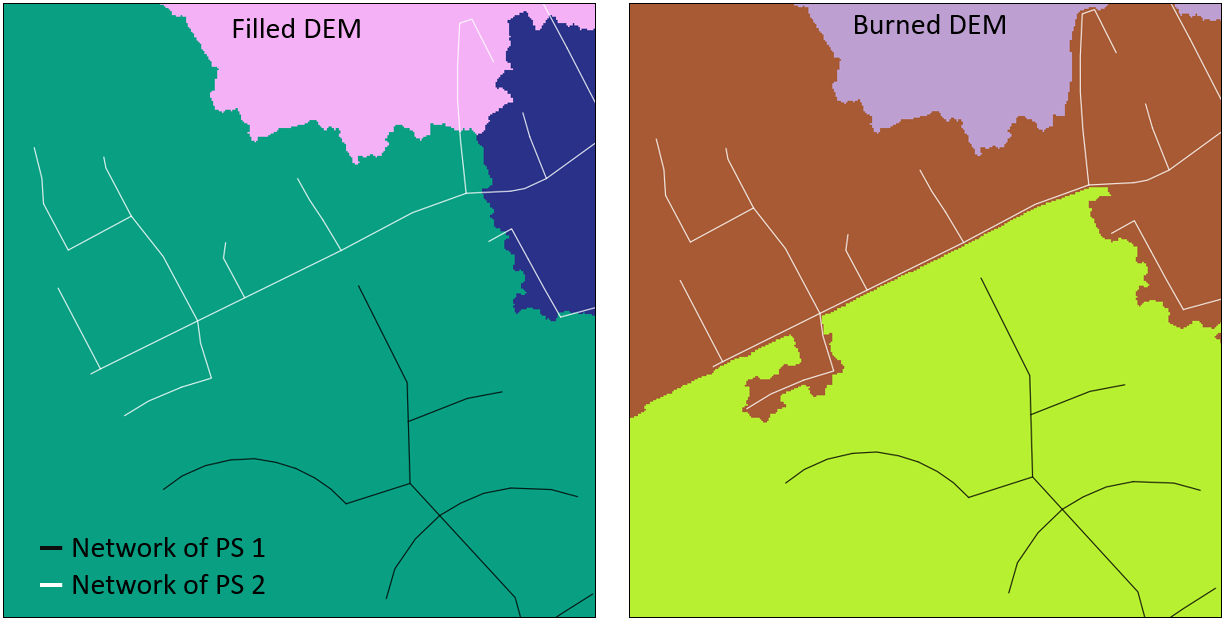
\includegraphics[scale=0.6]{figures/burnedxfilledDEM.png}
	\caption{Comparison of sewershed delineation using Filled and Burned DEM}
	\label{fig:filledxburned}
\end{figure}


, not all parts of.
The discretization in this study was DEM  Service area cadastral parcels.

Tell other options based on the network age, size, estimated defects, material, etc. 


Groundwater
         
DEM One of the first steps to model SWMMre are many ways to delineate a sewershed. The threshold level of discretization of the space domain. Each pipe section can have its own subcatchment 
          
          
         \textit{GRASS - v.clean} to split where streams intersect.
         \textit{QGIS - Merge Lines} To merge streams within the same layer. 
         \textit{QGIS - Split with lines} to split the sewershed polygon where the stream crosses.
        
        
        \subsubsection{Parameter Estimation}
    
    range of parameters are presented in each subsection of \ref{hydraulicmodel} chapter. 
    
    table \ref has the choice of parameters for all modules. The column \textit{Source} shows the references used to estimate the parameter as well as description of the data in previous section \ref{data}.
    
    Table
    
    \subsection{Synthetic Unit Hydrograph: RTK}
        
        \subsubsection{Parameter Estimation}
        
\section{Real-Time Simulations}